\documentclass[11pt]{article}

\usepackage[a4paper,margin=1in]{geometry}
\usepackage[T1]{fontenc}
\usepackage[utf8]{inputenc}
\usepackage{lmodern}
\usepackage{microtype}
\usepackage{graphicx}
\usepackage{booktabs}
\usepackage{listings}
\usepackage{xcolor}
\usepackage{hyperref}
\usepackage{cleveref}
\usepackage{tikz}
\usepackage{tabularx}
\usepackage{enumitem}
\usepackage{csquotes}
\usepackage[backend=biber,style=numeric,sorting=none]{biblatex}

\addbibresource{references.bib}

\usetikzlibrary{arrows.meta,positioning,shapes.geometric,fit}

\hypersetup{
  colorlinks=true,
  linkcolor=blue!50!black,
  citecolor=blue!50!black,
  urlcolor=blue!60!black,
  pdftitle={Improved CBMC Pipeline for OSEK-Aware Verification},
  pdfauthor={CBMC ISR/OSEK Research Branch}
}

\lstdefinestyle{reportstyle}{
  basicstyle=\ttfamily\small,
  breaklines=true,
  columns=fullflexible,
  frame=single,
  keepspaces=true,
  showstringspaces=false
}

\lstset{style=reportstyle}

\title{An Improved CBMC Pipeline for OSEK-Aware Verification and Targeted ISR Injection}
\author{CBMC ISR/OSEK Research Branch}
\date{\today}

\begin{document}

\maketitle

\begin{abstract}
OSEK applications mix task-level control flow, scheduler-visible API calls, event handling,
and asynchronous interrupt service routines (ISRs). A stock bounded model checking
workflow for C can reason about ordinary control flow, but it does not automatically know
that calls such as \texttt{ActivateTask}, \texttt{WaitEvent}, or \texttt{SetEvent} should
change scheduler state rather than behave like ordinary function bodies. Likewise, a broad
interrupt model can over-approximate the program by allowing ISR injection at many
irrelevant locations. This report documents an improved CBMC pipeline that addresses both
problems in a modular way. The first part adds an OSEK-aware \texttt{os-api} layer that
classifies recognized operating-system calls during symbolic execution and returns generic
next-step actions to \texttt{goto-symex}. The second part splits interrupt modeling into an
analysis-and-rewrite pipeline: \texttt{interleaving-analysis} computes a manifest of relevant
ISR insertion points from a GOTO model, and \texttt{aib} materializes those points as guarded
source-level calls in a copied project tree.

The checked-in benchmark artifacts show why this split matters. The large Trampoline
\texttt{alarms\_s1\_non} walkthrough covers 32 translation units and 7600 lines of source. The
scripted naive modeling path injects 747 ISR calls, while the checked-in targeted manifest
for the same case narrows the result to three ISR functions and six guarded call insertions,
which is a 99.2\% reduction in candidate call sites. At corpus level, the generated benchmark
report records 17 same-outcome comparable cases and 11 cases where the improved pipeline is
audited as the more faithful model. The trade-off is additional manifest, injection, and
recompile cost, but the pipeline documents a cleaner engineering boundary between scheduler
semantics, interference analysis, and source-to-source rewriting.
\end{abstract}

\section{Introduction}
\label{sec:introduction}

OSEK applications are not just sequential C programs with a few library calls. They combine
task-level control flow, scheduler-visible operating-system APIs, event synchronization, and
interrupt service routines (ISRs) whose interference is both asynchronous and highly
domain-specific. The OSEK/VDX operating-system specification models a single-processor,
resource-aware, event-driven execution environment with explicit task states, scheduling
policies, and a standard API surface for services such as \texttt{ActivateTask},
\texttt{TerminateTask}, \texttt{SetEvent}, and \texttt{WaitEvent}~\cite{osek_spec}. Real
RTOS code bases such as Trampoline make heavy use of exactly this execution model and are
therefore poor fits for a verification flow that assumes ordinary function-call semantics or
unstructured asynchronous interference~\cite{trampoline_repo}.

CBMC already offers a strong baseline for C verification. Its normal architecture builds a
GOTO model from source code, symbolically executes that model, and discharges the resulting
equation with a SAT or SMT solver~\cite{cbmc_architecture,cbmc_repo}. However, a stock
CBMC workflow leaves two important gaps for OSEK-style software.

First, scheduler-facing OS calls are semantically richer than ordinary C functions. Treating
\texttt{ActivateTask} or \texttt{ChainTask} as plain calls either loses the scheduling meaning
entirely or forces users to encode scheduler behavior manually inside harness code. Second, a
naive interrupt model can place ISR interference at many irrelevant source locations. That
kind of over-approximation may still be sound, but it creates unnecessary state-space growth
and can produce failures that are artifacts of the modeling style rather than of the program.

The branch documented in this report addresses both problems with a deliberately split design.
An \texttt{os-api} layer plugs into \texttt{goto-symex} so that recognized OSEK calls affect
symbolic scheduler state directly. A separate \texttt{interleaving-analysis} library then
computes a manifest of plausible ISR insertion points from an existing GOTO model, and an
independent \texttt{aib} rewriter materializes only those guarded calls in a copied project
tree. The resulting workflow is more modular than embedding every policy into one stage of the
toolchain, and it exposes a concrete JSON contract between static interference analysis and
source-to-source instrumentation.

This report is an implementation-facing paper-style summary of that pipeline. It rewrites the
seed material in \texttt{docs/reports/Introduction.pdf} and
\texttt{docs/reports/Background.pdf}, but treats the checked-in code as the source of truth
when the prose and implementation differ. The report makes three concrete contributions:

\begin{itemize}[leftmargin=1.5em]
  \item It explains how OSEK-aware symbolic execution is integrated into CBMC through
  command-line options, dispatcher logic, and a generic scheduler action interface.
  \item It documents the manifest-driven ISR pipeline, including target-function discovery,
  read/write-set analysis, candidate-line reporting, and guarded source rewriting.
  \item It summarizes the available benchmark evidence, including cases where the improved
  pipeline is slower, cases where it is audited as the more faithful model, and one Trampoline
  walkthrough that shows how aggressively the targeted manifest shrinks the naive ISR
  injection space.
\end{itemize}

The rest of the report proceeds from context to mechanism to evidence. \Cref{sec:background}
briefly reviews the OSEK execution model, the stock CBMC flow, and the main families of
interrupt-aware model checking. \Cref{sec:method} describes the improved pipeline in detail.
\Cref{sec:evaluation} summarizes the evidence available in the checked-in benchmark artifacts,
and \Cref{sec:discussion} closes with practical limitations that matter for future
maintenance.

\section{Background}
\label{sec:background}

\subsection{OSEK/VDX Task, Scheduler, and Event Semantics}

The seed introduction material is centered on an observation that still holds for the current
branch: OSEK applications are difficult to verify because task scheduling is explicit and API
driven rather than an afterthought. In OSEK/VDX, tasks have well-defined states, priorities,
and scheduling policies, and the operating system mediates transitions between those states
through standardized services~\cite{osek_spec}. Basic tasks move among suspended, ready, and
running states. Extended tasks add waiting behavior and event masks, which means APIs such as
\texttt{SetEvent}, \texttt{GetEvent}, \texttt{ClearEvent}, and \texttt{WaitEvent} modify both
control flow and visible state.

This matters because the scheduler is not nondeterministic in the same way as a generic
threading runtime. OSEK code frequently relies on explicit priorities, ready queues, and
preemption rules. The benchmark cases in this repository also use OIL metadata to define task
identities and priorities, so a verification flow that ignores the OIL configuration loses a
large fraction of the execution model before symbolic execution even begins.

\subsection{Baseline CBMC Architecture}

CBMC follows a standard three-stage structure~\cite{cbmc_architecture}. First, a front-end
and \texttt{goto-cc} convert source files into a GOTO program. Second,
\texttt{goto-symex} symbolically executes that model and emits an SSA-style equation. Third,
the solver backend discharges the equation and optionally reconstructs a counterexample trace.
This is a strong baseline for ordinary C verification because it already understands low-level
control flow, bit-precise data, and solver-backed safety checks.

\begin{figure}[t]
  \centering
  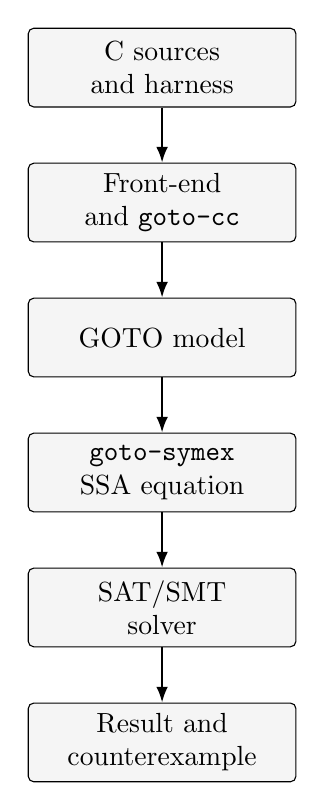
\begin{tikzpicture}[
  node distance=7mm,
  box/.style={
    draw,
    rounded corners=2pt,
    align=center,
    minimum width=34mm,
    minimum height=10mm,
    fill=gray!8
  },
  arrow/.style={-{Latex[length=2mm]},thick}
]
  \node[box] (src) {C sources\\and harness};
  \node[box,below=of src] (goto) {Front-end\\and \texttt{goto-cc}};
  \node[box,below=of goto] (model) {GOTO model};
  \node[box,below=of model] (symex) {\texttt{goto-symex}\\SSA equation};
  \node[box,below=of symex] (solver) {SAT/SMT\\solver};
  \node[box,below=of solver] (trace) {Result and\\counterexample};

  \draw[arrow] (src) -- (goto);
  \draw[arrow] (goto) -- (model);
  \draw[arrow] (model) -- (symex);
  \draw[arrow] (symex) -- (solver);
  \draw[arrow] (solver) -- (trace);
\end{tikzpicture}

  \caption{Baseline CBMC flow before the OSEK-aware and manifest-driven extensions described
  in this report.}
  \label{fig:baseline-cbmc}
\end{figure}

The limitation is not that CBMC lacks symbolic execution, but that a stock flow does not
automatically know which API calls are scheduler actions and which source statements are worth
instrumenting for ISR interference. Those are domain-specific choices. In this branch, they
are made explicitly instead of being hidden in monolithic harness code.

\subsection{Three Families of Interrupt-Aware Verification}

The background PDF reviews several styles of model checking for concurrent software. That
survey still gives a useful way to position the current implementation, provided the
terminology is updated to match the code in this repository.

\paragraph{Explicit-state exploration.}
Classical explicit-state tools such as SPIN build and traverse an explicit transition system,
which makes them a natural reference point for state-based concurrency reasoning~\cite{spin_site}.
Their strength is transparent control-state exploration; their weakness for this project is
that the OSEK scheduler and ISR placement policy still have to be modeled carefully to avoid
spurious interleavings.

\paragraph{SMT- and source-transformation-oriented flows.}
The benchmark corpora in this repository include artifacts from the CPROVER interrupt work and
from IntAbs~\cite{icbmc_site,intabs_repo}. Those families combine symbolic reasoning with
specialized source transformation or interrupt abstraction so that interleavings can be
restricted to relevant program points. The improved pipeline in this branch is closest to this
family, but it differs in two important ways: the OSEK scheduler semantics are integrated
inside CBMC rather than being left entirely to source transformation, and the static analysis
phase is cleanly separated from rewriting by a manifest boundary.

\paragraph{Sequentialization.}
Another well-known family translates concurrent behavior into a sequential model that can be
fed to an existing verifier. The background material emphasizes this as a scalability tactic
for branch-heavy applications. The current branch does not sequentialize the whole OSEK
system. Instead, it preserves CBMC's standard symbolic-execution core and inserts only the
scheduler and ISR modeling that are needed for the chosen project configuration.

These families motivate the design choices in \Cref{sec:method}. The branch documented here is
best understood as a hybrid engineering solution: keep CBMC's native GOTO and symex pipeline,
add OSEK semantics exactly where scheduler actions matter, and limit ISR modeling with a
static manifest rather than with blanket asynchronous injection.

\section{Methodology}
\label{sec:method}

\subsection{Overview of the Proposed Approach}

The method builds directly on the baseline CBMC architecture described in \Cref{sec:background}
and summarized in \Cref{fig:baseline-cbmc}. The goal is not to replace bounded model
checking, symbolic execution, or the solver stage. The goal is to construct a more accurate
checking model for OSEK/VDX applications before final verification. For ordinary C programs,
the baseline CBMC flow is often sufficient. For OSEK/VDX applications, however, the checking
model must also reflect how the deterministic scheduler, the ready queue, the task states,
and the standardized application interfaces (APIs) determine task execution order.

This section explains the proposed approach in four parts. First, it explains how the
checking model takes the OSEK/VDX scheduler into account. Second, it explains how the method
reduces unnecessary interleavings. Third, it explains how those two ideas are combined to
construct the final checking model. Fourth, it gives a short implementation note that maps
the methodology to the current realization in this branch.

Table~\ref{tab:method-comparison} provides the conceptual bridge from the baseline CBMC flow
in Section~2 to the methodology developed in the rest of this section. The comparison focuses
on the specific aspects that matter for OSEK/VDX verification: task execution order,
standardized APIs, interruption-related behaviour, unnecessary interleavings, and the
expected effect on verification accuracy.

\begin{table}[t]
  \centering
  \small
  \begin{tabularx}{\linewidth}{@{}>{\raggedright\arraybackslash}p{0.18\linewidth}>{\raggedright\arraybackslash}X>{\raggedright\arraybackslash}X@{}}
    \toprule
    Aspect & Baseline CBMC & Proposed Approach \\
    \midrule
    Task execution order & Follows ordinary program flow unless scheduler behaviour is
    encoded elsewhere. & Follows task states, the ready queue, and the deterministic
    scheduler inside the checking model. \\
    Standardized APIs & Can be treated as ordinary function effects if no OSEK/VDX-specific
    model is added. & Are interpreted as operations that may change task states, events, the
    ready queue, and therefore the next running task. \\
    Interruption-related behaviour & Broad asynchronous modelling can expose many possible
    interference points in the checking model. & Interruption-related behaviour is introduced
    only at program points where it can influence the checked execution. \\
    Unnecessary interleavings & Irrelevant interleavings may remain in the checking model and
    enlarge the verification problem. & Unnecessary interleavings are reduced before final
    bounded model checking. \\
    Expected accuracy outcome & May report a spurious bug or miss scheduler-dependent task
    execution order. & Aims to represent OSEK/VDX executions more faithfully while keeping
    CBMC's bounded model checking structure. \\
    \bottomrule
  \end{tabularx}
  \caption{Conceptual comparison between baseline CBMC and the proposed approach.}
  \label{tab:method-comparison}
\end{table}

The key point in Table~\ref{tab:method-comparison} is that the proposed approach does not
replace CBMC with a different verifier. It changes how the checking model is constructed
before final verification so that the solver is applied to a model that better reflects the
executions of OSEK/VDX applications.

To keep the discussion concrete, the remainder of this section uses one synthetic running
example. \textit{TaskControl} is a higher-priority task that waits for new sensor data.
\textit{TaskLogger} is a lower-priority task that can run while \textit{TaskControl} is
waiting. \textit{ISR\_Sensor} writes the shared sensor state and signals the event awaited by
\textit{TaskControl}. The example is intentionally small, but it is large enough to show the
three central decisions in the methodology: how task execution order is determined, how
unnecessary interleavings are reduced, and how the final checking model is built.

\subsection{Taking the OSEK/VDX Scheduler into Account}

The first methodological step is to represent the behaviour of the OSEK/VDX scheduler inside
the checking model. In an OSEK/VDX application, the next running task is not chosen by an
unstructured interleaving of threads. It is chosen by a deterministic scheduler that depends
on task states, priorities, events, and the ready queue. If the checking model ignores those
elements, the resulting task execution order no longer matches the execution order of the
application.

Listing~\ref{lst:running-example} shows the running example used throughout this section.
The example deliberately combines waiting, event signaling, shared-state update, and an
unrelated local computation so that each later methodological step can be tied back to the
same program.

\begin{lstlisting}[language=C,caption={Synthetic running example used throughout Section~3.},label={lst:running-example}]
volatile int sensor_ready = 0;
volatile int sensor_value = 0;

TASK(TaskControl)
{
  EventMaskType observed = 0;
  WaitEvent(EVENT_SENSOR_READY);
  GetEvent(TASK_ID_Control, &observed);
  if ((observed & EVENT_SENSOR_READY) != 0u && sensor_ready) {
    int sample = sensor_value;
    assert(sample >= 0);
  }
  ClearEvent(EVENT_SENSOR_READY);
  TerminateTask();
}

TASK(TaskLogger)
{
  int checksum = 0;
  checksum = checksum + 1;
  checksum = checksum * 2;
  TerminateTask();
}

ISR(ISR_Sensor)
{
  sensor_value = 7;
  sensor_ready = 1;
  SetEvent(TASK_ID_Control, EVENT_SENSOR_READY);
}
\end{lstlisting}

Table~\ref{tab:running-config} summarizes the intended execution context for this example.
The details are simple on purpose: \textit{TaskControl} begins as the running task,
\textit{TaskLogger} is already ready at a lower priority, and the interruption can make the
higher-priority task ready again by signaling the awaited event.

\begin{table}[t]
  \centering
  \small
  \begin{tabularx}{\linewidth}{@{}>{\raggedright\arraybackslash}p{0.22\linewidth}>{\raggedright\arraybackslash}p{0.22\linewidth}X@{}}
    \toprule
    Entity & Priority / type & Initial status and role \\
    \midrule
    \textit{TaskControl} & Higher-priority extended task & Running at the beginning of the
    path; waits for \texttt{EVENT\_SENSOR\_READY}; later reads the event state and the shared
    sensor value. \\
    \textit{TaskLogger} & Lower-priority task & Ready while \textit{TaskControl} is running;
    may execute while \textit{TaskControl} is waiting; performs only local computation in
    this example. \\
    \textit{ISR\_Sensor} & Interruption & Writes \texttt{sensor\_ready} and
    \texttt{sensor\_value}, then signals the event awaited by \textit{TaskControl}. \\
    \bottomrule
  \end{tabularx}
  \caption{Configuration summary for the running example.}
  \label{tab:running-config}
\end{table}

The central point is that the standardized APIs in
Listing~\ref{lst:running-example} cannot be treated as ordinary function effects. When
\textit{TaskControl} executes \texttt{WaitEvent}, the important effect is not simply that a
call occurs. The important effect is that the task may move from the running state to the
waiting state. Once that happens, \textit{TaskLogger} may become the next runnable task.
Later, when \textit{ISR\_Sensor} executes \texttt{SetEvent}, the event state changes and
\textit{TaskControl} may become ready again. Because \textit{TaskControl} has higher
priority, the deterministic scheduler may then dispatch it ahead of \textit{TaskLogger}.
The checking model must therefore represent state changes in the scheduler domain, not merely
ordinary control-flow changes in the current C function.

Table~\ref{tab:running-trace} is the output of this first methodological step. It shows how
the same source program leads to different verification states once the scheduler, the ready
queue, and the task states are represented explicitly in the checking model.

\begin{table}[t]
  \centering
  \footnotesize
  \begin{tabularx}{\linewidth}{@{}>{\raggedright\arraybackslash}p{0.07\linewidth}>{\raggedright\arraybackslash}p{0.20\linewidth}>{\raggedright\arraybackslash}p{0.23\linewidth}>{\raggedright\arraybackslash}p{0.16\linewidth}>{\raggedright\arraybackslash}p{0.11\linewidth}>{\raggedright\arraybackslash}X@{}}
    \toprule
    Step & Current context & Task states & Ready queue & Event state & Next dispatch decision \\
    \midrule
    0 & Start of path & \textit{TaskControl}: running; \textit{TaskLogger}: ready & \textit{TaskLogger} & Clear & Keep \textit{TaskControl} running \\
    1 & \textit{TaskControl} executes \texttt{WaitEvent} while the event is clear & \textit{TaskControl}: waiting; \textit{TaskLogger}: ready & \textit{TaskLogger} & Clear & Switch to \textit{TaskLogger} \\
    2 & \textit{TaskLogger} executes local computation & \textit{TaskControl}: waiting; \textit{TaskLogger}: running & Empty & Clear & Keep \textit{TaskLogger} running unless interrupted \\
    3 & \textit{ISR\_Sensor} writes shared state and signals the event & \textit{TaskControl}: ready; \textit{TaskLogger}: ready or preemptable & \textit{TaskControl}, \textit{TaskLogger} & Set & Preempt with \textit{TaskControl} \\
    4 & \textit{TaskControl} resumes, observes the event, and reads shared data & \textit{TaskControl}: running; \textit{TaskLogger}: ready & \textit{TaskLogger} & Set, then cleared & Keep \textit{TaskControl} running \\
    \bottomrule
  \end{tabularx}
  \caption{State evolution for the running example when the checking model tracks task states,
  the ready queue, and the event state explicitly.}
  \label{tab:running-trace}
\end{table}

Figure~\ref{fig:osek-sequence} summarizes the same causal chain at a higher level. The
figure is not a control-flow graph. It is a compact view of how a standardized API changes
task states and events, how those changes reach the ready queue, and how the deterministic
scheduler turns that information into the next task execution step in the checking model.

\begin{figure}[t]
  \centering
  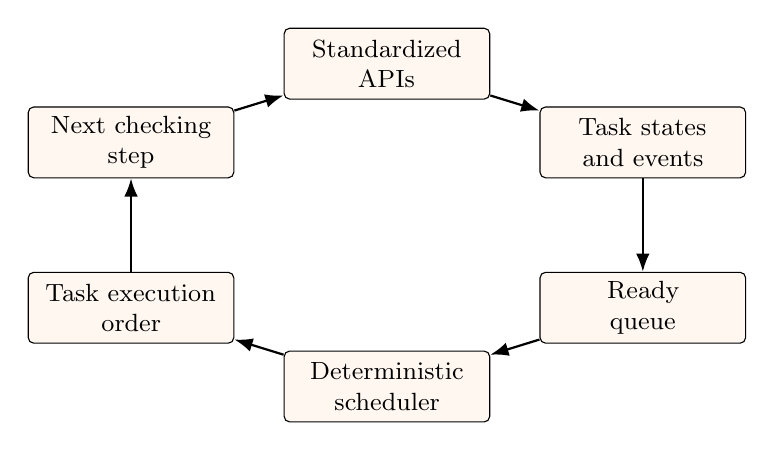
\begin{tikzpicture}[
  >=Latex,
  font=\small,
  box/.style={
    draw,
    rounded corners=2pt,
    align=center,
    text width=24mm,
    minimum height=9mm,
    inner sep=3pt,
    fill=orange!6
  },
  arrow/.style={->, thick}
]
  \node[box] (api) at (0,2.05) {Standardized\\APIs};
  \node[box] (state) at (3.25,1.05) {Task states\\and events};
  \node[box] (queue) at (3.25,-1.05) {Ready\\queue};
  \node[box] (sched) at (0,-2.05) {Deterministic\\scheduler};
  \node[box] (order) at (-3.25,-1.05) {Task execution\\order};
  \node[box] (step) at (-3.25,1.05) {Next checking\\step};

  \draw[arrow] (api) -- (state);
  \draw[arrow] (state) -- (queue);
  \draw[arrow] (queue) -- (sched);
  \draw[arrow] (sched) -- (order);
  \draw[arrow] (order) -- (step);
  \draw[arrow] (step) -- (api);
\end{tikzpicture}

  \caption{Conceptual cycle from standardized application interfaces (APIs) to task states,
  the ready queue, the deterministic scheduler, and the next checking step.}
  \label{fig:osek-sequence}
\end{figure}

Read clockwise, the cycle says the following. A standardized API such as \texttt{WaitEvent},
\texttt{GetEvent}, or \texttt{SetEvent} changes the scheduler-visible state of the
application. Those changes update the task states and the event information associated with
the affected tasks. The resulting state determines the contents of the ready queue. The ready
queue is then interpreted by the deterministic scheduler to determine task execution order.
That task execution order determines the next checking step, which may in turn lead to
another standardized API or another scheduler-relevant state update. Baseline CBMC follows
ordinary control-flow effects, whereas the proposed approach must also update task state and
scheduler state in the checking model.

In the running example, this means that the verification path should not simply continue with
the syntactically next statement after \texttt{WaitEvent}. Instead, the checking model should
represent that \textit{TaskControl} is blocked, that \textit{TaskLogger} may run while the
higher-priority task is waiting, and that \textit{ISR\_Sensor} can make
\textit{TaskControl} ready again. Only then does the task execution order in the
verification result reflect the execution order defined by the OSEK/VDX scheduler.

\subsection{Reducing Unnecessary Interleavings}

Taking the scheduler into account is not sufficient by itself. The second methodological step
is to reduce unnecessary interleavings in the checking model. Existing checking approaches for
concurrent software often consider a very broad set of asynchronous behaviours. In the
present setting, that can enlarge the verification problem and can also produce a spurious
bug when interruption-related behaviour is introduced at program points that are irrelevant to
the property being checked.

The key question is therefore not ``where could an interruption happen in general?'' The key
question is ``where can interruption-written state affect the checked execution?'' This is a
narrower and more useful question because it focuses the checking model on observable effects.
If interruption-written state cannot influence a later branch, a task-state transition, or a
property-relevant shared-data read, then representing interruption-related behaviour at that
point adds interleavings without improving accuracy.

The running example makes this distinction concrete. \textit{ISR\_Sensor} writes the event
state observed by \textit{TaskControl} and the shared variables \texttt{sensor\_ready} and
\texttt{sensor\_value}. Those writes matter near the points where \textit{TaskControl}
decides whether it should block, where it observes the signaled event, where it branches on
that information, and where it reads the shared sensor value. By contrast, the two checksum
updates inside \textit{TaskLogger} are purely local in this example. They do not observe the
event state, they do not change the ready queue, and they do not influence the later branch
or shared-data read that matter for the checked path.

Table~\ref{tab:selected-points} shows the output of this second methodological step. The
table is intentionally human-readable. It does not list raw artifact fields. It records only
the conceptual question answered by the analysis: which program points must retain
interruption-related behaviour because they can affect the checked execution?

\begin{table}[t]
  \centering
  \footnotesize
  \begin{tabularx}{\linewidth}{@{}>{\raggedright\arraybackslash}p{0.33\linewidth}>{\raggedright\arraybackslash}p{0.19\linewidth}>{\raggedright\arraybackslash}p{0.12\linewidth}X@{}}
    \toprule
    Program point in the running example & Depends on interruption-written state? & Keep / discard & Reason \\
    \midrule
    Immediately before \texttt{WaitEvent(EVENT\_SENSOR\_READY)} & Yes & Keep & The interruption can determine whether the task remains running or moves to the waiting state. \\
    Immediately before \texttt{GetEvent(TASK\_ID\_Control, \&observed)} & Yes & Keep & The returned event mask depends on whether the interruption has already signaled the awaited event. \\
    Immediately before the branch that checks \texttt{observed} and \texttt{sensor\_ready} & Yes & Keep & The branch condition depends directly on state written by the interruption. \\
    Immediately before the read of \texttt{sensor\_value} & Yes & Keep & The shared value read by \textit{TaskControl} is produced by the interruption. \\
    Immediately before \texttt{checksum = checksum + 1} in \textit{TaskLogger} & No & Discard & The computation is local to \textit{TaskLogger} and cannot observe interruption-written state in this example. \\
    Immediately before \texttt{checksum = checksum * 2} in \textit{TaskLogger} & No & Discard & This step is also local and does not affect task release, event state, or the later shared-data read. \\
    \bottomrule
  \end{tabularx}
  \caption{Conceptual selection result for interruption-relevant program points in the
  running example.}
  \label{tab:selected-points}
\end{table}

The point of Table~\ref{tab:selected-points} is not to predict the exact moment of every
interruption. The point is to keep only those program points where interruption-written state
can change the path explored by bounded model checking. Baseline CBMC with broad
asynchronous modelling may still explore both the kept and the discarded points. The
proposed approach keeps the first group and removes the second group from the final checking
model, which reduces unnecessary interleavings without discarding the scheduler-relevant
behaviour.

\subsection{Building the Final Checking Model}

The proposed approach combines the previous two ideas by separating two decisions that are
often mixed together. The first decision is analytical: identify the program points at which
interruption-related behaviour can influence the checked execution. The second decision is
constructive: build a new checking model that introduces interruption-related behaviour only
at those selected points.

This separation matters because the two decisions answer different questions. The analytical
step asks where interruption-written state can affect task execution order or a
property-relevant computation. The constructive step asks how to represent those effects in
the final checking model. Keeping those steps separate avoids a monolithic transformation in
which relevance and model rebuilding are entangled. As a result, the final checking model can
remain narrower than a blanket insertion of interruption-related behaviour at many unrelated
points.

For the running example, the analytical result can be summarized in the compact form shown in
Listing~\ref{lst:selected-summary}. This summary is the bridge between the two stages: it is
already specific enough to guide reconstruction, but it is still expressed in terms of the
checked path rather than in low-level artifact details.

\begin{lstlisting}[caption={Human-readable summary of the selected program points for the running example.},label={lst:selected-summary}]
Selected points
1. Before WaitEvent(EVENT_SENSOR_READY)
2. Before GetEvent(TASK_ID_Control, &observed)
3. Before the branch that checks observed and sensor_ready
4. Before the read of sensor_value

Excluded points
- The local checksum updates inside TaskLogger
\end{lstlisting}

Figure~\ref{fig:improved-pipeline} shows how the final checking model is then built. The
upper lane shows the baseline CBMC path. The lower lane shows the additional construction
stages used by the proposed approach before final bounded model checking.

\begin{figure}[t]
  \centering
  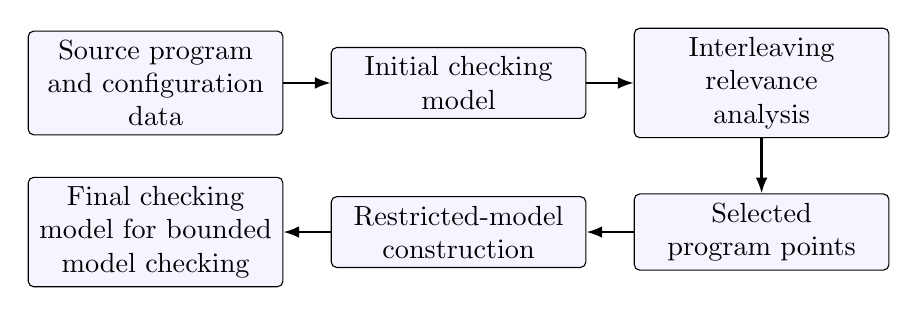
\begin{tikzpicture}[
  node distance=7mm and 6mm,
  box/.style={
    draw,
    rounded corners=2pt,
    align=center,
    text width=30mm,
    minimum height=9mm,
    fill=blue!4
  },
  arrow/.style={-{Latex[length=2mm]},thick}
]
  \node[box] (src) {Source program\\and configuration\\data};
  \node[box,right=of src] (gotocc) {Initial checking\\model};
  \node[box,right=of gotocc] (analysis) {Interleaving\\relevance\\analysis};
  \node[box,below=of analysis] (manifest) {Selected\\program points};
  \node[box,left=of manifest] (aib) {Restricted-model\\construction};
  \node[box,left=of aib] (cbmc) {Final checking\\model for bounded\\model checking};

  \draw[arrow] (src) -- (gotocc);
  \draw[arrow] (gotocc) -- (analysis);
  \draw[arrow] (analysis) -- (manifest);
  \draw[arrow] (manifest) -- (aib);
  \draw[arrow] (aib) -- (cbmc);
\end{tikzpicture}

  \caption{Baseline and improved checking-model construction. Numbered blocks indicate stages
  added by the proposed approach.}
  \label{fig:improved-pipeline}
\end{figure}

Conceptually, the upper lane starts from the original program and proceeds directly to model
construction, symbolic execution, and bounded model checking. The lower lane inserts four
additional responsibilities. The first added block builds a project-scoped view of the
program rather than a single straight-line execution view. The second added block identifies
where interruption-written state can affect the checked path. The third added block rebuilds
a restricted source-level checking model that retains interruption-related behaviour only at
those selected points. The fourth added block applies scheduler-consistent symbolic execution
so that standardized APIs change task states, the ready queue, and task execution order in a
way that matches OSEK/VDX semantics. This is the second major difference from baseline CBMC:
the proposed approach changes both where interruption-related behaviour appears and how the
resulting task execution order is interpreted during verification.

Listing~\ref{lst:restricted-checking-model} shows the output of the constructive step for the
running example. The guarded calls are part of the checking model, not part of the original
application program. They are placed only at the selected points. No such call is inserted
inside the local checksum updates of \textit{TaskLogger}, because those updates were excluded
as unnecessary interleavings in Table~\ref{tab:selected-points}.

\begin{lstlisting}[language=C,caption={Illustrative restricted checking model for the running example.},label={lst:restricted-checking-model}]
TASK(TaskControl)
{
  EventMaskType observed = 0;
  if (nondet_bool()) ISR_Sensor(0);
  WaitEvent(EVENT_SENSOR_READY);
  if (nondet_bool()) ISR_Sensor(0);
  GetEvent(TASK_ID_Control, &observed);
  if (nondet_bool()) ISR_Sensor(0);
  if ((observed & EVENT_SENSOR_READY) != 0u && sensor_ready) {
    if (nondet_bool()) ISR_Sensor(0);
    int sample = sensor_value;
    assert(sample >= 0);
  }
  ClearEvent(EVENT_SENSOR_READY);
  TerminateTask();
}

TASK(TaskLogger)
{
  int checksum = 0;
  checksum = checksum + 1;
  checksum = checksum * 2;
  TerminateTask();
}
\end{lstlisting}

The methodological role of Listing~\ref{lst:restricted-checking-model} is straightforward.
The checking model still admits interruption-related behaviour, but only at points where that
behaviour can change the execution being checked. This preserves the main advantage claimed
in Sections~1 and~2: fewer unnecessary interleavings without ignoring the OSEK/VDX
scheduler or the shared state written by interruptions.

\subsection{Implementation Note}

The current branch realizes this methodology with a small set of focused extensions rather
than a monolithic verifier rewrite. Table~\ref{tab:implementation-note} summarizes the role
of each concrete component and the artifact or checking-model effect it produces.

\begin{table}[t]
  \centering
  \small
  \begin{tabularx}{\linewidth}{@{}>{\raggedright\arraybackslash}p{0.26\linewidth}>{\raggedright\arraybackslash}X>{\raggedright\arraybackslash}X@{}}
    \toprule
    Component & What it consumes and does & What it produces \\
    \midrule
    \shortstack[l]{\texttt{goto-cc}\\extension} & Consumes the source program and configuration data, then
    builds the initial checking model while preserving the project-level view needed by the
    later analysis stage. & An initial checking model together with the project-scoped
    information needed to analyze interruption relevance. \\
    \shortstack[l]{\texttt{interleaving-}\\\texttt{analysis}} & Consumes the initial checking model and the designated
    interruption sources, then identifies program points where interruption-written state can
    affect the checked path. & A selection artifact describing the retained program points for
    restricted reconstruction. \\
    \shortstack[l]{\texttt{aib} with\\\texttt{lib-interleaving-block}} & Consumes the original project tree
    and the selection artifact, then rebuilds a restricted source-level checking model with
    guarded interruption calls only at the retained points. & A rewritten project view that is
    narrower than blanket interruption insertion. \\
    \shortstack[l]{\texttt{goto-symex} with\\\texttt{os-api}} & Consumes the restricted checking model and the
    OSEK/VDX configuration, then realizes the effects of standardized APIs on task states,
    events, the ready queue, and dispatch decisions during symbolic execution. & Scheduler-
    consistent symbolic states for final bounded model checking. \\
    \bottomrule
  \end{tabularx}
  \caption{Concrete realization of the methodology in the current branch.}
  \label{tab:implementation-note}
\end{table}

Figure~\ref{fig:improved-pipeline} uses these component boundaries implicitly. The added
blocks in the lower lane correspond, in order, to the project-scoped model-construction
extension around \texttt{goto-cc}, the separate \texttt{interleaving-analysis} stage, the
\texttt{aib} rewriting step built on \texttt{lib-interleaving-block}, and the
\texttt{goto-symex}/\texttt{os-api} realization of OSEK/VDX API effects during symbolic
execution.

Exact command-line spellings, manifest-field names, and concrete artifact formats are kept
out of the methodology body and collected in \Cref{sec:appendix}. That appendix is the right
place for interface-level details once the theoretical flow in this section is understood.

\section{Evaluation}
\label{sec:evaluation}

This section uses only the public benchmark families in the repository. Internal benchmark
families are intentionally excluded. The goal is not
to claim that the revised flow is always faster than the stock baseline. The checked-in
evidence shows the opposite in many cases because the manifest, injection, and rebuild stages
add cost. The evaluation instead answers two narrower questions:

\begin{enumerate}[leftmargin=1.5em]
  \item Do the public benchmark artifacts contain cases where the revised flow is judged more
  faithful than the stock asynchronous baseline?
  \item What cost is paid for that increase in accuracy?
\end{enumerate}

\subsection{Public Benchmark Scope}

The checked-in public report \texttt{check-src/benchmark.md} covers the five suites summarized
in \Cref{tab:public-suites}. Together they contribute 43 measured cases.

\begin{table}[t]
  \centering
  \small
  \begin{tabularx}{\linewidth}{@{}l c c X@{}}
    \toprule
    Suite & Cases & Headline-ready & Notes \\
    \midrule
    \texttt{icbmc-large} & 12 & yes & Larger i-CBMC-derived public cases. \\
    \texttt{icbmc-timeout-30m} & 4 & no & Public diagnostic cases kept outside the automatic
    suite. \\
    \texttt{icbmc-timeout-30m-blink-highmem} & 2 & no & Public high-memory blink cases. \\
    \texttt{icbmc-timeout-30m-logger-stable} & 4 & no & Public logger-focused diagnostic
    cases. \\
    \texttt{intabs-large} & 21 & yes & Larger public IntAbs-derived cases. \\
    \bottomrule
  \end{tabularx}
  \caption{Public benchmark suites used in this section.}
  \label{tab:public-suites}
\end{table}

\subsection{Public Correctness Summary}

The public subset has 43 measured cases. The correctness counts in
\Cref{tab:benchmark-summary} are recomputed for that public subset only.

\begin{table}[t]
  \centering
  \small
  \begin{tabularx}{\linewidth}{@{}l c X@{}}
    \toprule
    Benchmark verdict & Cases & Interpretation \\
    \midrule
    \texttt{same\_outcome\_comparable} & 17 & Stock and improved reached the same
    verification class. \\
    \texttt{improved\_correct} & 10 & The improved pipeline is audited as the more faithful
    model for the case. \\
    \texttt{no\_injection\_false} & 6 & The improved path reported no injection candidates
    even though state written by an interleaving function can still affect the main-reachable
    state. \\
    \texttt{needs\_manual\_review} & 3 & Output mismatch exists, but the current audit is not
    strong enough to choose a correct variant. \\
    \texttt{pending\_manual\_review} & 7 & Mismatch exists and no verdict rule has yet
    classified the case. \\
    \bottomrule
  \end{tabularx}
  \caption{Correctness summary for the public benchmark subset only.}
  \label{tab:benchmark-summary}
\end{table}

Two points stand out. First, the improved pipeline is not merely different from the stock
baseline; it is often audited as more faithful. Second, the benchmark report explicitly keeps
manual-review categories instead of silently forcing every mismatch into a win/loss label. That
is important engineering hygiene for an evolving verification branch.

\subsection{Representative Public Cases}

Three public cases illustrate the different ways in which the revised flow changes the
verification result.

\paragraph{\texttt{icbmc-timeout-30m-logger-stable / logger2-bug-conc-cprover}.}
The stock baseline reports \emph{VERIFICATION FAILED} in 56\,233 ms with 298.2 MB peak RSS,
while the improved pipeline reports \emph{VERIFICATION SUCCESSFUL} in 2\,017 ms with
16.6 MB peak RSS. The checked-in audit explains the difference directly: the stock async
baseline exposes a non-atomic asynchronous interleaving in the logger update, whereas the
improved pipeline checks the extracted interruption entry as one atomic region. This is a
clear public example of unnecessary interleavings producing a spurious bug.

\paragraph{\texttt{intabs-large / i8xx-tco-1}.}
The stock baseline reports \emph{VERIFICATION FAILED} in 1202 ms with 13.1 MB peak RSS, while
the improved pipeline reports \emph{VERIFICATION SUCCESSFUL} in 3395 ms with 15.3 MB peak RSS.
The benchmark audit again points to unnecessary interleavings in the stock model. The stock
run allows a non-atomic asynchronous interleaving, whereas the improved pipeline keeps the
interruption entry atomic and narrows the candidate set to three guarded interleavings. This
case shows the main accuracy gain of the revised flow even though the full measured time grows
from 1202 ms to 3395 ms.

\paragraph{\texttt{intabs-large / sc520wdt-2}.}
The stock baseline reports \emph{VERIFICATION SUCCESSFUL} in 1172 ms with 41.0 MB peak RSS.
The improved pipeline reports \emph{VERIFICATION FAILED} in 3559 ms with 16.7 MB peak RSS.
Here the improved pipeline injects closer/writer interleavings and reaches a violated
property that the stock baseline proves away. This is the opposite public pattern from the
previous two cases: the revised flow is slower, but it exposes an error trace that is not
reached by the stock model. The full measured time rises from 1172 ms to 3559 ms, but the
peak RSS drops from 41.0 MB to 16.7 MB.

Taken together, these public cases show the main cost of the revised flow. Even when the
verification phase itself is not dramatically slower, the extra manifest, injection, and
rebuild phases raise the full measured time. The public evidence therefore supports a clear
trade-off: the revised flow aims at a more accurate verification result, not at a faster one.

For the use case of this report, that trade is acceptable. The objective is not to outperform
the stock baseline on total wall-clock time, but to reduce unnecessary interleavings and make
bounded model checking more accurate for OSEK/VDX applications.

\section{Discussion and Limitations}
\label{sec:discussion}

The revised flow is deliberately conservative in some places and intentionally incomplete in
others. Those limitations are not incidental; they define where future work should focus.

\subsection{What the Current Design Gets Right}

The strongest engineering choice in the branch is the separation between the behaviours of
OSEK/VDX scheduler and the placement of interruption-related instrumentation. The task
execution order is determined during verification, while the candidate program points are
determined by an explicit analysis step and recorded in a manifest. This keeps the method
maintainable. A change to OSEK/VDX scheduling policy does not automatically require a change
to the instrumentation step, and a change to the candidate-line heuristics does not
automatically require a change to the verification core.

The evidence in \Cref{sec:evaluation} also suggests that the extra structure is not just
architecturally neat; it matters to outcomes. The benchmark report contains multiple cases in
which the improved pipeline is audited as the more faithful model even though it is slower.

\subsection{Current Analysis Limits}

\begin{itemize}[leftmargin=1.5em]
  \item \textbf{Source-file-driven target discovery.} Interleaving functions are selected from
  an explicit source-file list. If the relevant interruption file is not part of the build, the
  analysis cannot discover it.
  \item \textbf{Global-write-centric conflict rule.} Candidate lines are derived from globals
  written by the interleaving function and read or written by the main verification path. This keeps
  the rule simple, but it ignores purely read-side interactions by the interleaving function.
  \item \textbf{\texttt{.c}-only candidate filtering under project scope.} When project-root
  filtering is enabled, candidate recording is restricted to \texttt{.c} files under the root.
  Generated or indirect artifacts outside that slice are ignored.
  \item \textbf{Hand-written manifest IO.} Both the manifest writer and the \texttt{aib}
  reader are hand-coded. There is no schema version field, which makes coordinated changes
  brittle.
\end{itemize}

\subsection{Current OSEK Model Limits}

\begin{itemize}[leftmargin=1.5em]
  \item \textbf{Partial OIL subset.} The parser currently handles the fields needed by the
  implemented scheduling rules: \texttt{TASK}, \texttt{PRIORITY}, \texttt{SCHEDULE},
  \texttt{AUTOSTART}, \texttt{TYPE}, and \texttt{EVENT\_MASK}.
  \item \textbf{AUTOSTART is metadata, not boot behavior.} The configuration records
  \texttt{AUTOSTART}, but the current flow still expects explicit task activation from the
  harness or runtime stubs.
  \item \textbf{\texttt{WaitEvent} is an approximation.} The implementation models the block /
  no-block decision and wake-up dispatch, but not every possible continuation detail of the
  full operating-system behaviour.
  \item \textbf{API coverage is intentionally narrow.} The current branch focuses on task and
  event services relevant to the public benchmarks. Resource, alarm, and interruption-related
  APIs beyond this subset are not yet modeled through the same boundary.
\end{itemize}

\subsection{Performance Trade-offs}

The benchmark report consistently shows that the revised flow pays an overhead tax. Even
public cases add a manifest phase, an injection phase, and a rebuild. Larger cases can still
be worth that cost when the stock baseline either misses a real bug or invents one through
unnecessary interleavings, but the branch is not yet an optimization pass.

This suggests a practical reading of the current status: the branch is already useful as a
more accurate bounded model checking workflow, but not yet as a drop-in faster replacement for
stock CBMC. Improving analysis precision without paying so much orchestration cost is a
natural next step.

\section{Conclusion}
\label{sec:conclusion}

This report documented a CBMC-based bounded model checking flow for OSEK/VDX applications.
The central problem is accuracy: if the deterministic scheduler is ignored, many unnecessary
interleavings of tasks may be superfluously checked and may result in a spurious bug. The
revised flow addresses that problem by taking the behaviours of OSEK/VDX scheduler into
account and by restricting interruption-related instrumentation through an explicit manifest.

The checked-in public benchmark evidence supports that choice. The revised flow is often
slower because it adds analysis, instrumentation, and rebuild phases, but it is audited as the
more faithful model in meaningful public cases. In particular, it removes unnecessary
interleavings that produce spurious bugs and reaches some error traces that are not reached by
the stock baseline.

The remaining work is also clear. The supported OSEK/VDX subset can be widened, the manifest
contract can be made more robust, and the candidate-line rule can be made less dependent on a
simple global-write heuristic. Even in its current form, however, the branch demonstrates a
practical path toward more accurate bounded model checking for OSEK/VDX applications.


\appendix
\section{Appendix: Concrete Interfaces}
\label{sec:appendix}

\subsection{OSEK/VDX Checking Options}

The methodology in Section~3 refers to OSEK/VDX-specific model construction without listing
its command-line spellings. The following schematic command shows the documented options for
selecting the OSEK/VDX checking model and the corresponding OIL configuration file.

\begin{lstlisting}[caption={Schematic OSEK/VDX option usage.}]
cbmc main.c --os-api osek --osek-oil app.oil
\end{lstlisting}

\subsection{Example \texttt{goto-cc} Invocation}

The following command illustrates the public project-mode flow on the
\texttt{i8xx-tco-1} benchmark tree. It records the project root, names the interruption
source file explicitly, and emits an interleaving manifest.

\begin{lstlisting}[caption={Example project-mode interleaving analysis command.}]
goto-cc \
  check-src/benchmark-sources/intabs/cases/i8xx-tco-1/improved-pipeline/main.c \
  check-src/benchmark-sources/intabs/cases/i8xx-tco-1/improved-pipeline/isr_define/isr.c \
  --interleaving-project-root \
    check-src/benchmark-sources/intabs/cases/i8xx-tco-1/improved-pipeline \
  --interleaving-source-files \
    check-src/benchmark-sources/intabs/cases/i8xx-tco-1/improved-pipeline/isr_define/isr.c \
  --interleaving-output \
    check-src/benchmark-sources/intabs/cases/i8xx-tco-1/interleaving_pipeline.json \
  -o check-src/benchmark-sources/intabs/cases/i8xx-tco-1/i8xx-tco-1.out
\end{lstlisting}

\subsection{Example \texttt{aib} Invocation}

\begin{lstlisting}[caption={Example AIB rewrite command.}]
aib \
  check-src/benchmark-sources/intabs/cases/i8xx-tco-1/improved-pipeline \
  check-src/benchmark-sources/intabs/cases/i8xx-tco-1/interleaving_pipeline.json \
  out/i8xx-tco-1_injected \
  out/i8xx-tco-1_injected/interleaving_pipeline_effective.json
\end{lstlisting}

\subsection{Illustrative Guarded Call}

The restricted checking model is created by inserting guarded interruption calls only at the
selected program points. The example below is illustrative rather than benchmark-specific.

\begin{lstlisting}[caption={Illustrative guarded interruption call.}]
if (nondet_bool()) isr1(0);
\end{lstlisting}

\subsection{Documented Selection-Artifact Fields}

\begin{table}[H]
  \centering
  \small
  \begin{tabularx}{\linewidth}{@{}lX@{}}
    \toprule
    Field & Meaning \\
    \midrule
    \texttt{project.project\_root} & Root directory used for path scoping and
    report-path relativization. \\
    \texttt{project.interleaving\_source\_files} & Source files whose functions are treated
    as interleaving functions. \\
    \texttt{project.translation\_units} & Effective build inputs associated with the initial
    checking model that produced the selection artifact. \\
    \texttt{interleaving[*].name} & Interleaving function identifier recorded for rewriting. \\
    \texttt{interleaving[*].write\_global\_var} & Global symbols that the interleaving
    function may write. \\
    \texttt{interleaving[*].line\_added\_block\_with\_file} & Project-relative file and line
    pairs where guarded calls may be inserted. \\
    \bottomrule
  \end{tabularx}
  \caption{Documented fields of the selection artifact used between analysis and rewriting.}
  \label{tab:manifest-schema}
\end{table}

\subsection{Manifest Excerpt}

The manifest below is a schematic excerpt showing only the documented public fields. It
illustrates how project metadata and interleaving candidates are separated.

\begin{lstlisting}[caption={Schematic manifest excerpt.}]
{
  "project": {
    "project_root": "/path/to/check-src/benchmark-sources/intabs/cases/i8xx-tco-1/improved-pipeline",
    "interleaving_source_files": ["isr_define/isr.c"],
    "translation_units": [
      "main.c",
      "isr_define/isr.c"
    ]
  },
  "interleaving": [
    {
      "name": "isr1",
      "write_global_var": ["<global_1>", "<global_2>"],
      "line_added_block_with_file": [
        { "file": "main.c", "line": [<line_a>, <line_b>] }
      ]
    }
  ]
}
\end{lstlisting}

This schema is the compatibility boundary between \texttt{interleaving-analysis} and
\texttt{aib}; any field change must be implemented on both sides.


\printbibliography

\end{document}
